\documentclass[runningheads]{llncs}

\usepackage{listings}
\usepackage{enumitem}

\usepackage[T1]{fontenc}

\usepackage{graphicx}

%% %%%%%%%%%%%%%%%%%%%%%%%%%%%%%%%%%%%%%%%%%%%%%%%%%%%%%%%%%%%%%%%%%%%%%%%%%%
%% New commands 

\usepackage{xcolor}
\usepackage{tcolorbox}

\usepackage{amsmath,amssymb}
\usepackage{cleveref}

% Commands for TODOS
\newcommand{\nb}[2]{\fcolorbox{gray}{yellow}{\bfseries\sffamily\scriptsize#1}{\sf\small$\blacktriangleright$\textit{#2}$\blacktriangleleft$}}
\newcommand\todo[1]{\nb{Todo}{#1}}

\newcommand{\missref}{\fcolorbox{gray}{red}{\bfseries\sffamily\scriptsize\textcolor{white}{REF}} }

% Commands for TODOs
\newcommand{\alcides}[1]{{\nb{Alcides}{#1}}}
\newcommand{\chris}[1]{{\nb{Chris}{#1}}}
\newcommand{\miguel}[1]{{\nb{Miguel}{#1}}}
\newcommand{\ricardo}[1]{{\nb{Ricardo}{#1}}}
\newcommand{\paulo}[1]{{\nb{Paulo}{#1}}}


\begin{document}

\title{Formalization and Runtime Verification of Invariants for
Robotic Systems}

\author{Ricardo Cordeiro\inst{1} \and
%Paulo Canelas\inst{1,2} \and
Alcides Fonseca\inst{1} \and
Christopher S. Timperley\inst{2}}

\authorrunning{Cordeiro et al.}

\institute{Faculdade de Ciências da Universidade de Lisboa,
Lisboa, Portugal \and
Carnegie Mellon University, Pittsburgh, PA}

\maketitle

\begin{abstract}
    Robotic systems are critical in today's society. A potential failure in a robot may have extraordinary costs, not only financial but can also cost lives.
    Current practices in robot testing are vast and involve methods like simulation, log checking, or field testing. However, current practices often require human monitoring to determine the correctness of a given behavior. Automating this analysis can not only relieve the burden from a high-skilled engineer but also allow for massive parallel executions of tests that can detect behavioral faults in the robots. These faults could otherwise not be found due to human error or a lack of time.
    We have developed a Domain Specific Language to specify the properties of robotic systems in the Robot Operating System (ROS). Developer written specifications in this language compile to a monitor ROS module that detects violations of those properties in runtime. We have used this language to express the temporal and positional properties of robots, and we have automated the monitoring of some behavioral violations of robots in relation to their state or events during a simulation.

\keywords{Robotics \and Domain-specific language \and Runtime Monitoring \and Error detection.}
\end{abstract}


\section{Introduction}

Robotics already have a significant impact on our current society. Due to their broad practicality, the quality of software running on robots should be extremely important to us. However, robotic Systems are non-deterministic, mainly because robots interact directly with the real world. Testing software in such environments is complex, as many variables can change, and verifying the success of a task or movement may not be possible from the robot's perspective, and external monitoring may be required.

The Robot Operating System (ROS)~\cite{quigley2009ros} is an open-source framework with a vast collection of libraries, interfaces, and tools designed to help build robot software. ROS provides an abstraction between hardware and software that helps developers easily connect the different robot components through messages sent through communication channels (\textit{topics}).

Current practices in testing robot software mainly involve field testing, simulation testing, and log checking and require a human to analyze the robot's behavior to determine whether the behavior is correct.

An invariant represents a property that holds through the execution of the system. Having a set of invariants for a robotic system and asserting them at runtime makes it able to prove the correctness of the system. Research on invariant checking~\cite{zizyte2021importance} shows that a considerable amount of bugs on autonomous robotic systems can be avoided when representing safety violations of systems and monitoring them.

Due to the unforeseen circumstances mentioned when executing robotic systems, runtime monitoring, although sometimes time-consuming, may be advantageous when identifying errors in these systems. However, implementing a form of runtime monitoring adds load to the simulation. Therefore, not demanding excessive resources is essential when taking this approach. Some challenges in implementing such mechanisms are mentioned in the cited paper~\cite{stadler2022towards}.

Similar work on runtime monitoring that integrates with ROS already exists. ROSMonitoring~\cite{ferrando2020rosmonitoring} can monitor and log errors at the level of \textit{topic} malfunctioning, but it seems unable to express more high-level properties, which is the objective of this work. ROSRV~\cite{huang2014rosrv} although able to express more high-level specifications, it is highly complex and, in some way, hard for non-expert users to work with. An intuitive domain-specific language will allow a broader set of users to specify a robotic system's properties.

This work aims to provide developers with a way to verify their robotic systems' temporal and positional properties automatically. We propose the introduction of a domain-specific language for developers to express their relevant properties. The given properties compile into monitors that can be used in simulation to ensure the correctness of the system. The language was designed from the point of view of ROS developers and tries to abstract the underlying Linear Temporal Logic (LTL)~\cite{pnueli1977temporal}~\cite{dwyer1998property} system, allowing properties to reason about native ROS constructs, like \textit{topics}, \textit{messages} and simulation information. Thus, it is possible to express properties that relate the internal information of the system with the corresponding information in the simulator.

We have developed a compiler for the language that generates a ROS module that monitors an existing project. The module listens to relevant information from both the robot's components and the simulator. If a property violation occurs, it provides a detailed error message to the user.


\section{Motivational Example}

Let us consider an autonomous car developer wanting to express that its system always stops when near a stop sign. The following example presents a property defined in the language that specifies the intended behavior of the developer.


\vspace{2mm}
\texttt{after\_until robot.distance.stop\_sign < 1, robot.distance.stop\_sign > 1, eventually robot.velocity == 0}
\vspace{2mm}

\textit{Translating into natural language, the property states in the first section that after the robot's distance to the stop-sign is below the value of 1 in the simulator, and in the second section that up until the distance is again above 1, then in the third section the robot velocity will eventually be equal to 0.}
\vspace{2mm}

The specified property compiles to a Python file capable of running as a ROS node. The node listens only to relevant topics and performs the computations to verify the specified property.

\begin{figure}
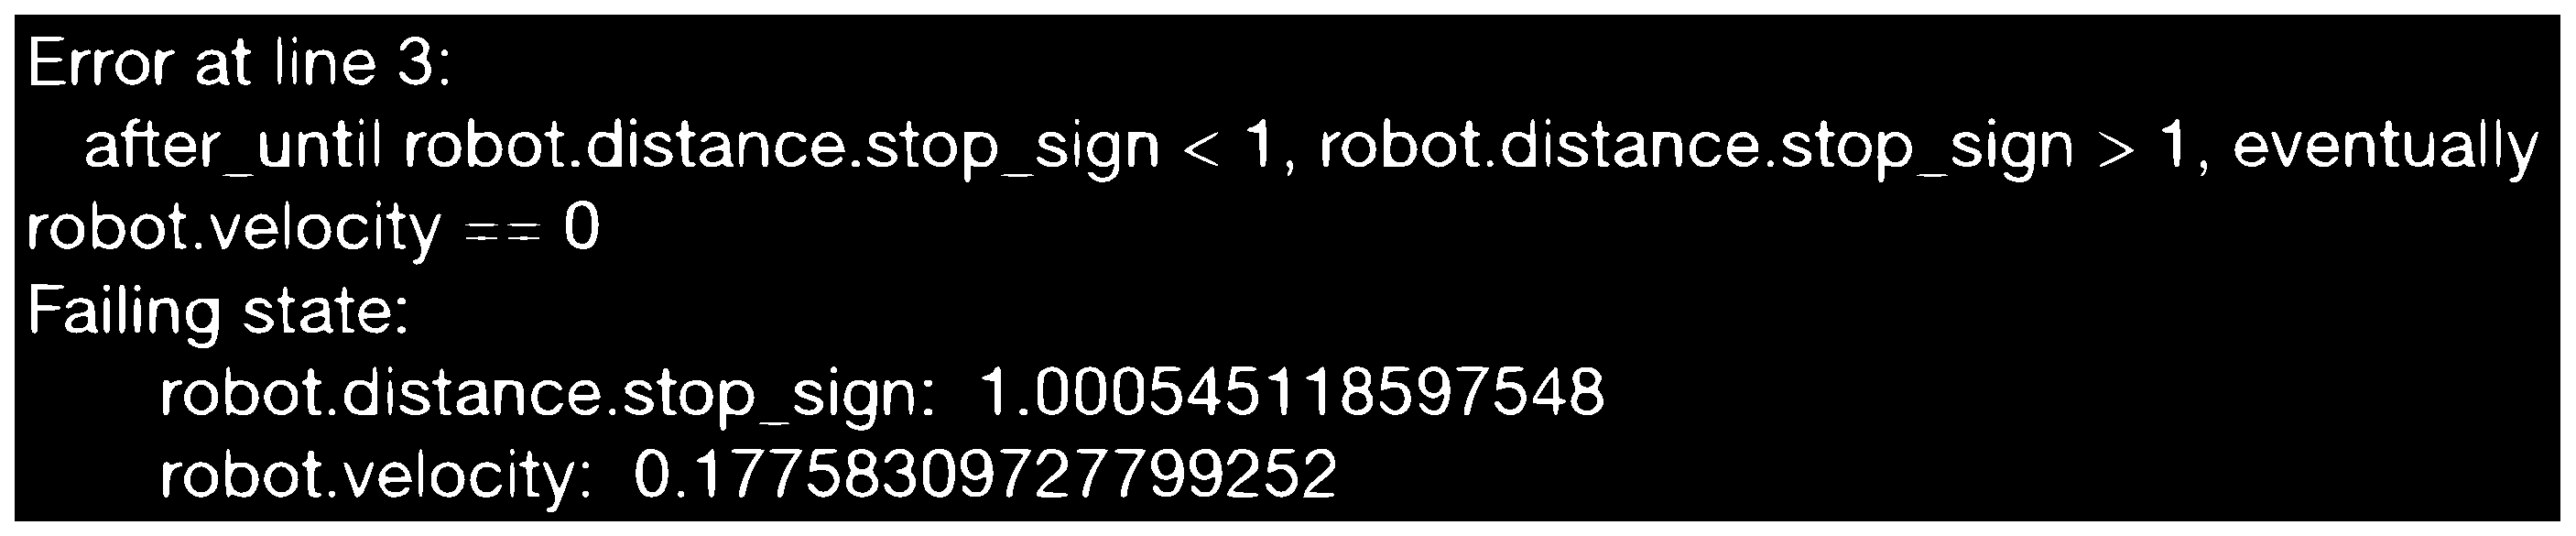
\includegraphics[width=\textwidth]{error.eps}
\caption{Example of the displayed error when the robot does not stop at the stop sign.} \label{fig1}
\end{figure}

The flow of the process of monitoring a robotic system is described as follows:

\begin{enumerate}[label=(\roman*)]
    \item \textbf{Property formalization:} the developer describes in the DSL the properties of the robotic system one wants to monitor in a \texttt{.txt} file extension.
    \item \textbf{Compilation:} The specified properties are compiled, and a python file is generated capable of running as a ROS node.
    \item \textbf{Monitoring:} The node can be run whenever testing the system and will listen to pertinent topics and perform the computations needed to verify the specified properties.
\end{enumerate}


\section{Specification Language for Robotics Properties}

The domain-specific language relies on an adaptation of LTL to express temporal relations of and between simulation objects (section 3.1). The DSL has shortcuts to express the absolute values of certain useful concepts of objects in a simulation in order to make it usable (section 3.2). The DSL allows the declaration of robots' relevant topics (section 3.3). And finally, the DSL allows modeling of a whole robot's specific \textit{topics} (section 3.4).

\subsection{Temporal Keywords}

We consider not only LTL basic operators but also some common shortcuts for useful combinations of such operators, like \textit{after\_until}, used in the previous example.

\begin{itemize}
\item {\bfseries always X} - X has to hold on the entire subsequent path;
\item {\bfseries never X} - X never holds on the entire subsequent path;
\item {\bfseries eventually X} - X eventually has to hold somewhere on the subsequent path;
\item {\bfseries after X, Y} - after the event X is observed, Y has to hold on the entire subsequent path;
\item {\bfseries until X, Y} - X holds at the current or future position, and Y has to hold until that position. At that position, Y does not have to hold anymore;
\item {\bfseries after\_until X, Y, Z} - after the event X is observed, Z has to hold on the entire subsequent path up until Y happens. At that position, Z does not have to hold anymore;
\end{itemize}

\noindent It is also possible to reference previous states of variables, using \lstinline|@{X, -y}|, representing the value of variable \lstinline|X| at time \lstinline|-y|.

\subsection{Simulation primivitives}

To support comparing the internal state of the robotic system with the environment, we provide basic primitives in the language to refer to the simulation environment:

\begin{itemize}
\item {\bfseries X.position} - The position of the robot in the simulation;
\item {\bfseries X.position.y} - The position in the y axis of the robot in the simulation. Also works for x and z;
\item {\bfseries X.distance.Y} - The absolute distance between two objects in the simulation. For the x and y axis;
\item {\bfseries X.distanceZ.Y} - The absolute distance between two objects in the simulation. For the x, y, and z axis;
\item {\bfseries X.velocity} - The velocity of an object in the simulation. This refers to linear velocity;
\item {\bfseries X.velocity.x} - The velocity in the x axis of an object in the simulation. This refers to linear velocity;
\item {\bfseries X.localization\_error} - The difference between the robot's perception of its position and the actual position in the simulation;
\end{itemize}


\subsection{Topic declaration}

In order to relate robot components with the simulation, the developer can declare the relevant \textit{topic}.

\textit{The variable robot\_position was declared with the type Odometry.pose.pose.position and is linked to the topic /odom;}

\vspace{2mm}

\texttt{decl robot\_position /odom Odometry.pose.pose.position}


\subsection{Model robots}

A set of specific topics can be modeled for the robot, like \textit{position} or \textit{velocity}. The compiler will use these to call specific functions that need this information from the robot's perspective.

\vspace{2mm}

\texttt{model robot1:}

\texttt{    position /odom Odometry.pose.pose.position}

\texttt{    ;}

\vspace{2mm}

\texttt{never robot1.localization error > 0.002}


\section{Examples}

To validate the expressive power of our language, we present examples of expressions inspired by real-world scenarios.


\subsection{Vehicle Maximum Speed}

Some robots have a maximum safe speed at which they can move. Sometimes this limit is imposed by law, but some other times by physical constraints.


\textit{The robot velocity will never be above 2 for the duration of the simulation;}

\vspace{2mm}

\texttt{never robot.velocity > 2.0}

\subsection{Follow the Leader}

The first robot being above 1 velocity implies that the second robot is at least at 0.8 distance from the first robot. Up until the first robot reaches a particular location;

\vspace{2mm}

\texttt{until (robot1.position.x > 45 and robot1.position.y > 45), always (robot1.velocity > 1 implies robot2.distance.robot1 > 0.8)}


\subsection{Drone height rotors control}

After a drone is at a certain altitude, both rotors always have the same velocity up until the drone decreases to a certain altitude.

\vspace{2mm}

\texttt{decl rotor1\_vel /drone\_mov/rotor1 Vector3.linear.x}

\texttt{decl rotor2\_vel /drone\_mov/rotor2 Vector3.linear.x}

\vspace{2mm}

\texttt{after\_until drone.position.z > 5, drone.position.z < 5, rotor1\_vel == rotor2\_vel}


\section{Conclusion}

The proposed approach can express some interesting scenarios that developers care about. We are expanding our examples to include bugs found~\footnote{\url{https://github.com/robust-rosin/robust}} in real work projects and from a survey, we are conducting with expert developers. Our development is available online~\footnote{\url{https://ricardocajo.github.io/error-monitor-ros-gazebo}} for those that want to experiment with it. We also intend on expanding the primitives with more simulator information or with the possibility of integrating sensors for supporting field testing in alternative to simulation.


\bibliographystyle{ieeetr}
\bibliography{references}

\end{document}
